% =============================================================================
% FILE NAME : 00_introduction.tex
% DEPARTMENT: University of Tuebingen
% AUTOR     : Tom Schammo
% =============================================================================
% CONTENT   : Include for chapter "Introduction"
% =============================================================================


Rust \cite{rustlang} is a somewhat new language,
with their very first release in early 2012 \cite{rust_releases}.
But the 1.0 alpha release was only in early 2015 \cite{rust_releases}
with the full 1.0 release following a few months later in Mai of the same year \cite{rust_releases}.
C, as a comparison has been used as early as the 1970s.\\
But Rust has been gaining in popularity \cite{rust_popularity} over the last few years, however
due to its relatively 'young' age there still are huge gaps when it comes to software support and available libraries.
So in my thesis I'll improve upon the Rust ecosystem by expanding upon the thesis of Raphael Vogelgsang \cite{rust_pulp}
and implementing support for the UltraTrail \cite{ultratrail} AI accelerator.
\\\\
This thesis is structured as follows:
The chapter \ref{cha:fundamentals} will provide a fundamental overview of RISC-V, 'Embedded AI', (embedded) Rust and microphone technology.\\
Chapter \ref{cha:related_work} covers previous work on the PULPissimo, and goes a bit into the UltraTrail architecture.
Finally, it covers the state of keyword spotting in the industry.
It briefly goes into its use cases and then covers one of them a little more in depth.
The concept of the thesis is covered in \ref{cha:concept}.
That chapter briefly introduces what I'm trying to do in my thesis.
After that it covers the microphones used and finally goes into the tests that I have used
to assess the functionality of the UltraTrail and microphone drivers.
\todo{rest der kapitel}


% \section{Umfang der Arbeit}
% ,,Dies ist eine der meistgestellten Fragen. Natürlich verbirgt sich dahinter die Vermutung, die erzielbare Note sei – gutachterabhängig – mit der Seitenzahl korreliert (vgl. Abb.~\ref{fig:graph}). Nur
% wie? Linear, normalverteilt, nach dem Gesetz vom abnehmenden Grenznutzen?
% Tatsächlich kommt es auf die Qualität Ihrer Resultate an. Wenn Sie mit Ihrer Arbeit das Collatz-Problem, auch bekannt als Ulams Vermutung, widerlegen können, genügt eine Seite Inhalt mit dem Hinweis, die Zahl, welche die Vermutung widerlegt, befinde sich auf der beigefügten CD.
%
% \begin{figure}[htb]
%   \centering
%   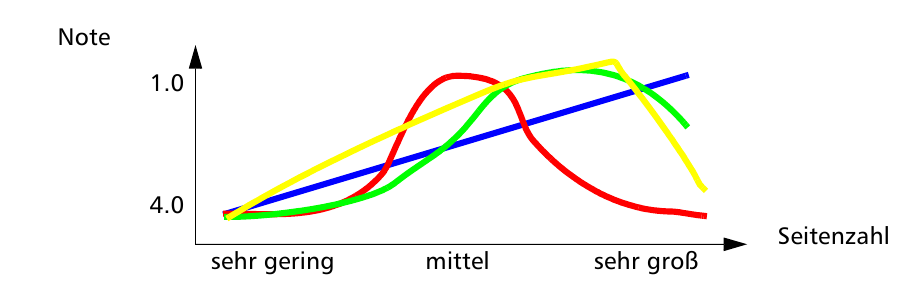
\includegraphics[width=0.9\textwidth]{figures/note_page.png}
%   \caption[Verteilung: Seitenanzahl-Note]{Welcher Verteilung folgt die Note als Funktion der Seitenzahl?}
%   \label{fig:graph}
% \end{figure}
%
% Für alle, die nicht so viel Glück haben, soll die folgende Tabelle \ref{tab:tabelle-2} auf Seite \pageref{tab:tabelle-2} als Richtschnur
% dienen. Dabei wurden Anhänge, Inhalts- und Abbildungsverzeichnisse sowie Stichwortverzeichnisse (sofern überhaupt vorhanden, da nicht üblich) nicht gerechnet.Bedenken Sie, dass Ihr Gutachter das alles gründlich lesen soll, der Zweitgutachter es vielleicht
% auszugsweise lesen muss. Formulieren Sie deshalb knapp und auf den Punkt, vermeiden Sie Wiederholungen („Wir kommen nochmal auf das schwierige Problem der Softwareauswahl aus
% Kapitel zwei zu sprechen, wo wir feststellten, dass ...“).
% Längliche Passagen, etwa Programmstücke, Teile der Dokumentation, sehr lange Zitate (etwa ein Beweis, ein Gerichtsurteil, ein Zeitschriftenartikel im Wortlaut), Messreihen usw.
% verbannen Sie in den Anhang (mit der Gewissheit, dass das kaum jemand gründlich lesen wird).
% Aber auch bei den Anhängen ist weniger oft mehr. Noch umfangreichere Teile lassen sich auf
% eine CD brennen, die der Arbeit beigefügt wird; allerdings ist umstritten, ob ein Gutachter sich
% diese anschauen muss.
%
% \begin{table}[tb]
%   \centering
%   \begin{tabular}{cccc}
%     \toprule
%     \textbf{Art der Arbeit} & \textbf{Untergrenze} & \textbf{Obergrenze} & \textbf{Anmerkung} \\
% 		\midrule
%     Bachelor & 35 & 65 & ideal $\leq$ 50 \\
%     Master & 50 & 85 & ideal $\leq$ 70 \\
%     \bottomrule
%   \end{tabular}
%   \caption{Empfehlung zur Seitenanzahl der Arbeit}
%   \label{tab:tabelle-2}
% \end{table}
%
%
% Weil das Vorwort, der erste Abschnitt der Einleitung und die abschließende Zusammenfassung mit Ausblick immer gründlich gelesen werden, sollten Sie darauf besonderes Augenmerk
% legen. In der Regel schreibt man die Einleitung und das Vorwort auch erst, wenn der restliche
% Teil einschließlich Zusammenfassung (Fazit) steht, Spötter nennen das die Anpassung des
% Anforderungsprofils an das tatsächlich erzielte Resultat.
% Zuletzt ein Rat, wenn der Umfang der Arbeit erkennbar zu groß wird. So wie bei Seminarvorträgen Schnellersprechen das Problem eines zu umfangreichen Folienprogramms nicht
% lösen kann, so wenig lässt sich mit typografischen Mitteln (kleinerem Font, engeren Zeilenabständen, breiteren Spalten) wesentlich Platz ohne Verlust an Lesbarkeit gewinnen. Sie kommen
% nicht umhin, größere Teile der Arbeit zu streichen oder wesentlich zu straffen.
% Dafür bieten sich oft die Kapitel an, in denen Sie den mühsamen Prozess der Lösungsfindung
% einschließlich aller notwendigen Vorarbeiten und Diskussionen mit dem Anwender dokumentiert haben. Hinter solchen längeren Beschreibungen steckt der verständliche Wunsch, der Gutachter möge honorieren, dass Sie unglaublich mit dem Auftraggeber, der undurchsichtigen
% Software, dem abstürzenden Computer u.a.m. kämpfen mussten und vieles zunächst nicht so
% funktionierte, wie gedacht.
% Leser sind aber wie Restaurantgäste, Gutachter ähneln Gourmetkritikern. Sie sind mitleidslos und schauen nur auf den Teller vor sich. Sie wollen nichts davon wissen, dass frische Seezunge heute enorm schwierig zu beschaffen war und der Jungkoch sich am Gratin die Finger
% verbrannt hat. Halten Sie Ihre Schwierigkeiten in einem ehrlich geschriebenen 10-Zeilen-Abschnitt der Zusammenfassung fest, als Teil der Selbstreflektion, die immer zu einer
% Abschlussarbeit gehört, und streichen Sie schweren Herzens Teile der Entwicklungssaga.''
